\section{Überlegungen für die Multilane-Szenarios}
\label{sec:ueberlegungen-multilane}

Aufgrund zweier Fehler\footnote{siehe \url{https://github.com/LightJason/AgentSpeak/issues/47} und \url{https://github.com/LightJason/AgentSpeak/issues/50}} im Agenten-Framework, die bis zum Termin dieser Arbeit nicht behoben wurden, war es mir nicht möglich, auch belastende Tests für die Mehrspurszenarien durchzuführen.

Dennoch liegen theoretische Überlegungen und in Teilen getestete praktische Vorarbeiten vor, die in diesem Kapitel präsentiert werden sollen.





\subsection{Veränderung der Agentenpläne}
\label{agentplan-multilane}

Für die Simulation mehrspuriger Fahrbahnen müssen dem Agentenverhalten lediglich zwei Pläne für das Ausscheren (Pull-out) und das Einscheren (Pull-in) hinzugefügt werden.
%Für das komplette Listing siehe \cref{lst:multilane}.
\sa{own: add listing multilane}

\begin{minipage}[hptb]{0.95\textwidth}
\begin{lstlisting}[style=asl, 
                   keywords={!pullout,!pullin}, 
                   keywords={[2]}, 
                   keywords={[3]}, 
                   caption={Auszug aus Agentenscript: multi lane-Version},
                   label={lst:multilane-auszug}]      
!cruise.

// --- start all other plans ---
+!cruise <-
    !accelerate;
    !decelerate;
    !linger;
    !pullout
    !pullin
    !cruise
.\end{lstlisting}
\end{minipage}

\paragraph*{\texttt{pullout}-Plan}
\hfill \\
Der Plan für das Ausscheren ist mit insgesamt fünf Bedingungen versehen.

\begin{enumerate}
	\itemsep0em
	\item Befindet sich das Fahrzeug nicht auf der am weitesten linken Fahrspur?
	\item Ist in der aktuellen Spur Verkehr voraus?
	\item Ist Verkehr in der Spur, in die gewechselt werden soll, nicht näher?
	\item Befindet sich Verkehr direkt links neben dem Fahrzeug?
	\item Ist der rückwärtige Verkehr auf der Überholspur ausreichend weit entfernt?
\end{enumerate}

Die erste Bedingung ist zwingend notwendig, da sonst keine Spur zum hineinwechseln vorhanden wäre.
Die Auslösung eines Kollisionsereignisses wäre in der Simulation die Folge.
\\
Die zweite Bedingung macht den Ausschervorgang erst nötig. 
Wäre die aktuelle Spur nicht blockiert, könnte auf ihr weitergefahren werden.
\\
Ein Spurwechsel ist nur sinnvoll, wenn auf der zukünftigen Spur mindestens genauso viel Platz nach vorn ist, wie auf der aktuellen. 
Dem trägt Bedingung 3 Rechnung.
\\
Durch die Unterteilung des Sichtfeldes in vier Sektoren, siehe \cref{sec:unterteilung-sichtfeld}, wurde die vierte Bedingung notwendig.
\\
Um den nachfolgenden Verkehr nicht zu behindern, ist die fünfte Regel zu beachten.

Durch die o.g. Fehler im Framework ist die gleichzeitige Auswertung aller Bedingungen unmöglich.
\\
Bei keiner der Bedingungen ist es möglich, diese wegzulassen oder mit einer anderen zusammenzufassen, ohne dass unerwünschtes Verhalten auftritt.

Würden zum Beispiel die Bedingungen 2 und 3 zusammengefasst und nur auf forwärtigen Verkehr (in beiden Spuren) geprüft, so würde dies zwar der Bedingung \enquote{nicht schlechter} für die Überholspur genügen, aber jedes überholende Fahrzeug würde zum Auslösen der Bedingung führen.
Dies sogar in übergroßen Maße, da die Entfernung sehr gering ist.



%\subsection{Testläufe des Mehrspurmodells}
%\label{test-multilane}
%
%Da die Ausführung der erdachten Logik nicht funktioniert, wurde überlegt, das Verhalten mit Alternativen/Workarounds herzustellen.
%
%Eine Idee war, die zweite und dritte Bedingung zusammenzufassen.
%Dies hätte aber zur Folge, dass
%
%IDEE
%Für den Zweispurfall könnte man die zweite und die dritte Bedingung zusammenfassen.
%NO RISK, NO FUN -- try not looking left.




\subsection{Zufälligkeit des Aus- und Einscherens}
\label{sec:pullout-pullin}

Um unterschiedliche Verhalten beim Überholen im Autobahnverkehr abbilden zu können, benötigt man einen Mechanismus, Wahrscheinlichkeiten für jew. eine der Handlungen zu generieren.

Dieses wurde u.a. in \cite{dat-ba} anhand des \enquote{Social-Force-Vehicle-Modells} versucht. 
Der dort erarbeitete Ansatz scheint jedoch das gewünschte Verhalten übermäßig zu bevorteilen.

Für den Anreiz zum Spurwechsel nach links (Pull-out) oder rechts (Pull-in) genügt im Zweispurfall die Berechnung der jeweiligen Wahrscheinlichkeit.
Die Wahrscheinlichkeit, die Spur zu halten, wäre jeweils die Gegenwahrscheinlichkeit.
\\
Für Szenarien mit mehr als zwei Spuren ist eine Exklusivität (XOR) der beiden Ereignisse zu gewährleisten.
Hier könnte die Wahl auf die Alternative mit der größeren Wahrscheinlichkeit fallen bei exakter Gleichheit würde es Sinn machen, aufgrund des zu überholenden Verkehrs und des Verbotes des rechts Überholens, den Spurwechsel nach links zu präferieren.

\paragraph*{Wahrscheinlichkeitsfunktion} 
\hfill \\
Für eine Bestimmung von Wahrscheinlichkeiten für diesen Zweck erscheint die logistische Funktion  
\begin{center}
$ f(x) = \frac{1}{1 + e^{-x}} $ 
\end{center}
siehe \cite{logistic-function}, eine Sigmoid-Funktion, ein geeigneter Kandidat. 
Ihr Definitionsbereich sind alle Zahlen in $ \mathbb{R} $ und ihr Wertebereich liegt zwischen 0 und 1.
\\
Die Grundfunktion steigt im Intervall $ [-5; 5] $ ziemlich rasch von nahe 0 auf nahe 1.
Dies kann durch Streckung der Funktion etwas abgemildert werden.
So verläuft z.B. 
\begin{center}
$ f(x) = \frac{1}{1 + e^{-\frac{1}{2}x}} $ 
\end{center}
weniger steil und hat den für diesen Zweck sinnvoll nutzbaren Intervall $ [-10; 10 ] $.
Für Werte außerhalb dieses Intervalles ergibt sich eine kleine von Null, bzw. große von Eins verschiedene Wahrscheinlichkeit.

\paragraph*{Wahrscheinlichkeit des Ausscherens (Pull-out)} 
\hfill \\
Für das Ausscheren wurden die folgende Zusammenhänge, bezogen auf ein vorausfahrendes Fahrzeug, erkannt:
\begin{itemize}
    \itemsep0em
    \item Abstand $ \searrow $  $ \Longrightarrow $ Ausscherwunsch $ \nearrow $ (und umgekehrt)
    \item relative Geschwindigkeit $ \nearrow $ $ \Longrightarrow $ Ausscherwunsch $ \nearrow $ (und umgekehrt)
\end{itemize}

Es galt sinnvolle Werte zu finden und diese auf den o.g. Intervall zu normieren.

Für den Abstand $ s $ wurde die Grenze der Zone der Nahortientierung/Handlung, siehe \cref{sec:sichtweite} - 110 m - und ein Punkt, an dem nach Möglichkeit spätestens ein Überholvorgang eingeleitet sein sollte - 50 m - gewählt.
\\
Dies führt zu der Funktion
\begin{center}
$ f(s) = -\frac{s}{3} + \frac{80}{3} $
\end{center}
Somit ergibt sich für die Überholwahrscheinlichkeit in Abhängigkeit vom Abstand zum vorausfahrenden Fahrzeug $ p_{po}(s) $
\begin{center}
$ p_{po}(s) = \frac{1}{1 + e^{-\frac{1}{2}f(s)}} $
\end{center}

\noindent
Für die relative Geschwindigkeit $ v_{rel} $ wurden die Grenzen bei 0 und 25 km/h festgelegt.
Ab 0 km/h bzw. darunter ist kein Überholen mehr nötig.
Für die obere Grenze wurde das Verhalten auf Landstraßen, siehe \cite[S. 27]{ueberholgeschwindigkeit}, auf den Autobahnverkehr übertragen.
\\
Dies führt zu der Funktion 
\begin{center}
$ f(v_{rel}) = \frac{4 v_{rel}}{5} - 10 $
\end{center}
Für die Überholwahrscheinlichkeit in Abhängigkeit von der relativen Geschwindigkeit zum vorausfahrenden Fahrzeug $ p_{po}(v_{rel}) $ ergibt sich
\begin{center}
$ p_{po}(v_{rel}) = \frac{1}{1 + e^{-\frac{1}{2}v_{rel}}} $
\end{center}

\noindent
Eine Kombination der beiden Gleichungen und Normierung auf den Intervall $ [0; 1] $
\begin{center}
$ p_{po} = \frac{1}{2}(p_{po}(s) + p_{po}(v_{rel})) = \frac{1}{2}p_{po}(s) + \frac{1}{2}p_{po}(v_{rel}) $
\end{center}
liefert die Wahrscheinlichkeit für das Ausscheren $ p_{po} $.

Es ergibt sich eine Funktionskurve mit drei erkennbaren Plateaubildungen um die Werte 0, 0,5 und 1, siehe \cref{figure:kurve-ueberholwahrscheinlichkeit}.
Die Darstellung erfolgt in den Intervallen  $ [0; 1] $ für die Wahrscheinlichkeit, $ [ 40; 120 ] $ für den Abstand und $ [ -5; 30 ] $ für die relative Geschwindigkeit.

\begin{figure}[hptb]
 \centering
 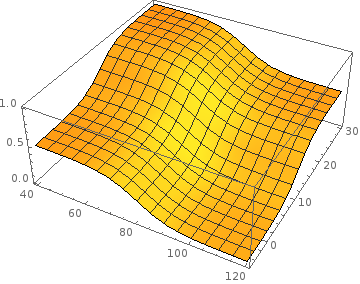
\includegraphics[width=0.5\textwidth]{kurve-ueberholwahrscheinlichkeit}
 \caption[Funktionskurve für die Ausscherwahrscheinlichkeit]
 		 {Plateaubildung der Funktionskurve der Ausscherwahrscheinlichkeit}
 \label{figure:kurve-ueberholwahrscheinlichkeit}
\end{figure} 

Hier wären die beiden Wahrscheinlichkeiten gleich gewichtet (Faktor $ \frac{1}{2} $). Eine unterschiedliche Gewichtung kann durch Faktoren, welche in Summe 1 ergeben müssen, herbeigeführt werden.

\paragraph*{Wahrscheinlichkeit des Einscherens (Pull-in)} 
\hfill \\
Eine ähnliche Herangehensweise ist für das Einscheren möglich.
Hier müssten allerdings sowohl der vorausfahrende Verkehr $ T_{f} $, als auch der rückwärtige Verkehr $ T_{b} $ beachtet werden. 
Aufgrund der fehlenden Möglichkeit eines Tests, wird hier nur das Konzept umrissen.

\begin{itemize}
    \itemsep0em
    \item Abstand $ T_{f} $ $ \nearrow $ $ \Longrightarrow $ Einscherdrang $ \nearrow $ (und umgekehrt)
    \item relative Geschwindigkeit $ T_{f} $ $ \searrow $ $ \Longrightarrow $ Einscherdrang $ \nearrow $ (und umgekehrt)
    \item Abstand $ T_{b} $ $ \nearrow $ $ \Longrightarrow $ Einscherdrang $ \nearrow $ (und umgekehrt)
    \item relative Geschwindigkeit $ T_{b} $ $ \nearrow $ $ \Longrightarrow $ Einscherdrang $ \nearrow $ (und umgekehrt)
\end{itemize}

Beim Zusammenfassung der entstehenden einzelnen Wahrscheinlichkeiten kann ebenfalls wieder über Faktoren eine individuelle Gewichtung vorgenommen werden.
